\section{Computador} 
\label{computer}
Esta pesquisa se propõe a construir um computador clássico (ilustrado a baixo), de forma que se possa por em prática a teoria estudada, possibilitando uma maior compreensão sobre a temática. Tendo em vista a metodologia de Project based learning – em que se incentiva a aprendizagem a partir da aplicação de conhecimentos e de habilidades através da experiência. Assim, o presente capítulo se debruça em detalhar o processo prático da construção do computador, sendo possível implementar as teorias, anteriormente vistas, na prática. Desta maneira, qualquer pessoa interessada, será capaz de construir seu próprio dispositivo, vivenciando o processo de Project based learning. 

\vspace{1cm}
\begin{figure}[H] \centering 
  \makebox[\textwidth][c]{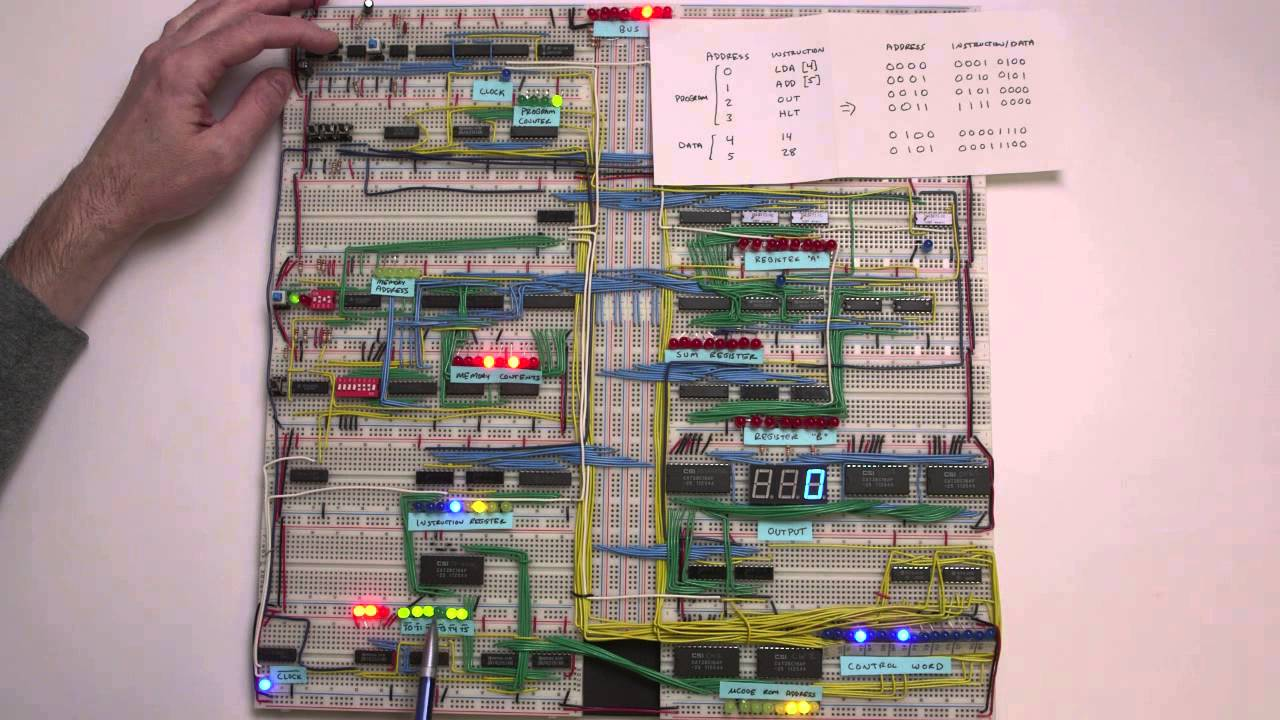
\includegraphics[width=0.8\textwidth]{breadboard_computer.jpg}}
  \caption{\label{breadboard_computer} Protótipo a ser implementado, imagem do site \href{https://eater.net/}{eater.net}} 
\end{figure}

A implementação deste computador já foi iniciada, porém, há sérias desconfianças de que o prazo ainda restante seja adequado para sua finalização, maiores detalhes sobre o tema são apresentados no cronograma \ref{updated_timeline}. Apesar de todos os esforços, ainda que com prazos apertados, para o cumprimento dessa construção, ainda, tem-se que a implementação física dos modelos contribui para a academia, uma vez que professores poderão usufruir dos mesmos como ferramenta didática, agregando para a compreensão da teoria ao aproximá-la da prática.

O projeto do computador aqui referenciado pode ser dividido em diversas partes, pois como qualquer computador clássico convencional, cada parte especifica contribui a sua maneira para a operacionalidade de todo o sistema. Essas partes são separados em módulos, os quais são ilustrados na figura \ref{breadboard_computer}, sendo que esses módulos fomam a ULA (Unidade Lógica Aritmética) e a UC (Unidade de Controle) – conforme descrito na arquitetura von Neumann (capítulo \ref{classic_comp}):

Conforme pode ser observado na figura \ref{breadboard_computer}, os módulos são organizados como: Clock, Registradores, Unidade Logica Aritmética, Memoria RAM, Contador e Registrador de Output.

A seguir, cada seção traz a funcionalidade e atual implementação de cada uma das partes, módulos, do computador.



% No entanto, apesar desse capítulo ter sido reservado para descrever o passo a passo de como desenvolver um computador clássico apenas com portas lógicas simples, devido a alguns problemas esclarecidos na seção \ref{problems} não foi possível concluí-lo. Porém, de forma a manter a metodologia de Project based Learning, foi desenvolvido um sistema operacional que permitiu colocar em prática o conteúdo estudado ao implementar um processo de boot, usando o assembly intelx86. Além disso pode-se produzir um emulador de assembly, de forma didática e publicado na web,  a fim de contribuir com material para academia. Ademais, sugere-se que a proposta original seja adiada e implementada em um trabalho futuro. 

% Apesar desta alteração no projeto, optou-se por compartilhar o conteúdo já produzido no início do processo de construção. 

\subsection{Módulos}
Para facilitar a compreensão e também o desenvolvimento do computador, este capítulo será dividido em alguns subcapítulos, cada qual abordando uma parte do computador.

\subsubsection{Clock}
O clock do computador é uma parte essencial para o seu funcionamento. Este tem a função de sincronizar todas as operações. A ação mais rápida que o computador consegue executar é equivalente a uma vibração do seu clock. No módulo desenvolvido, três clocks se fazem presentes. Assim o computador pode operar em três modos distintos, sendo eles, controlado por um potenciômetro – vibrando em uma frequência constante –, controlado pelo operador – a cada click no botão o modulo emite uma vibração –, e sempre ligado – assim passando o mais rápido possível por cada operação.

\vspace{1cm}
\begin{figure}[H] \centering 
  \makebox[\textwidth][c]{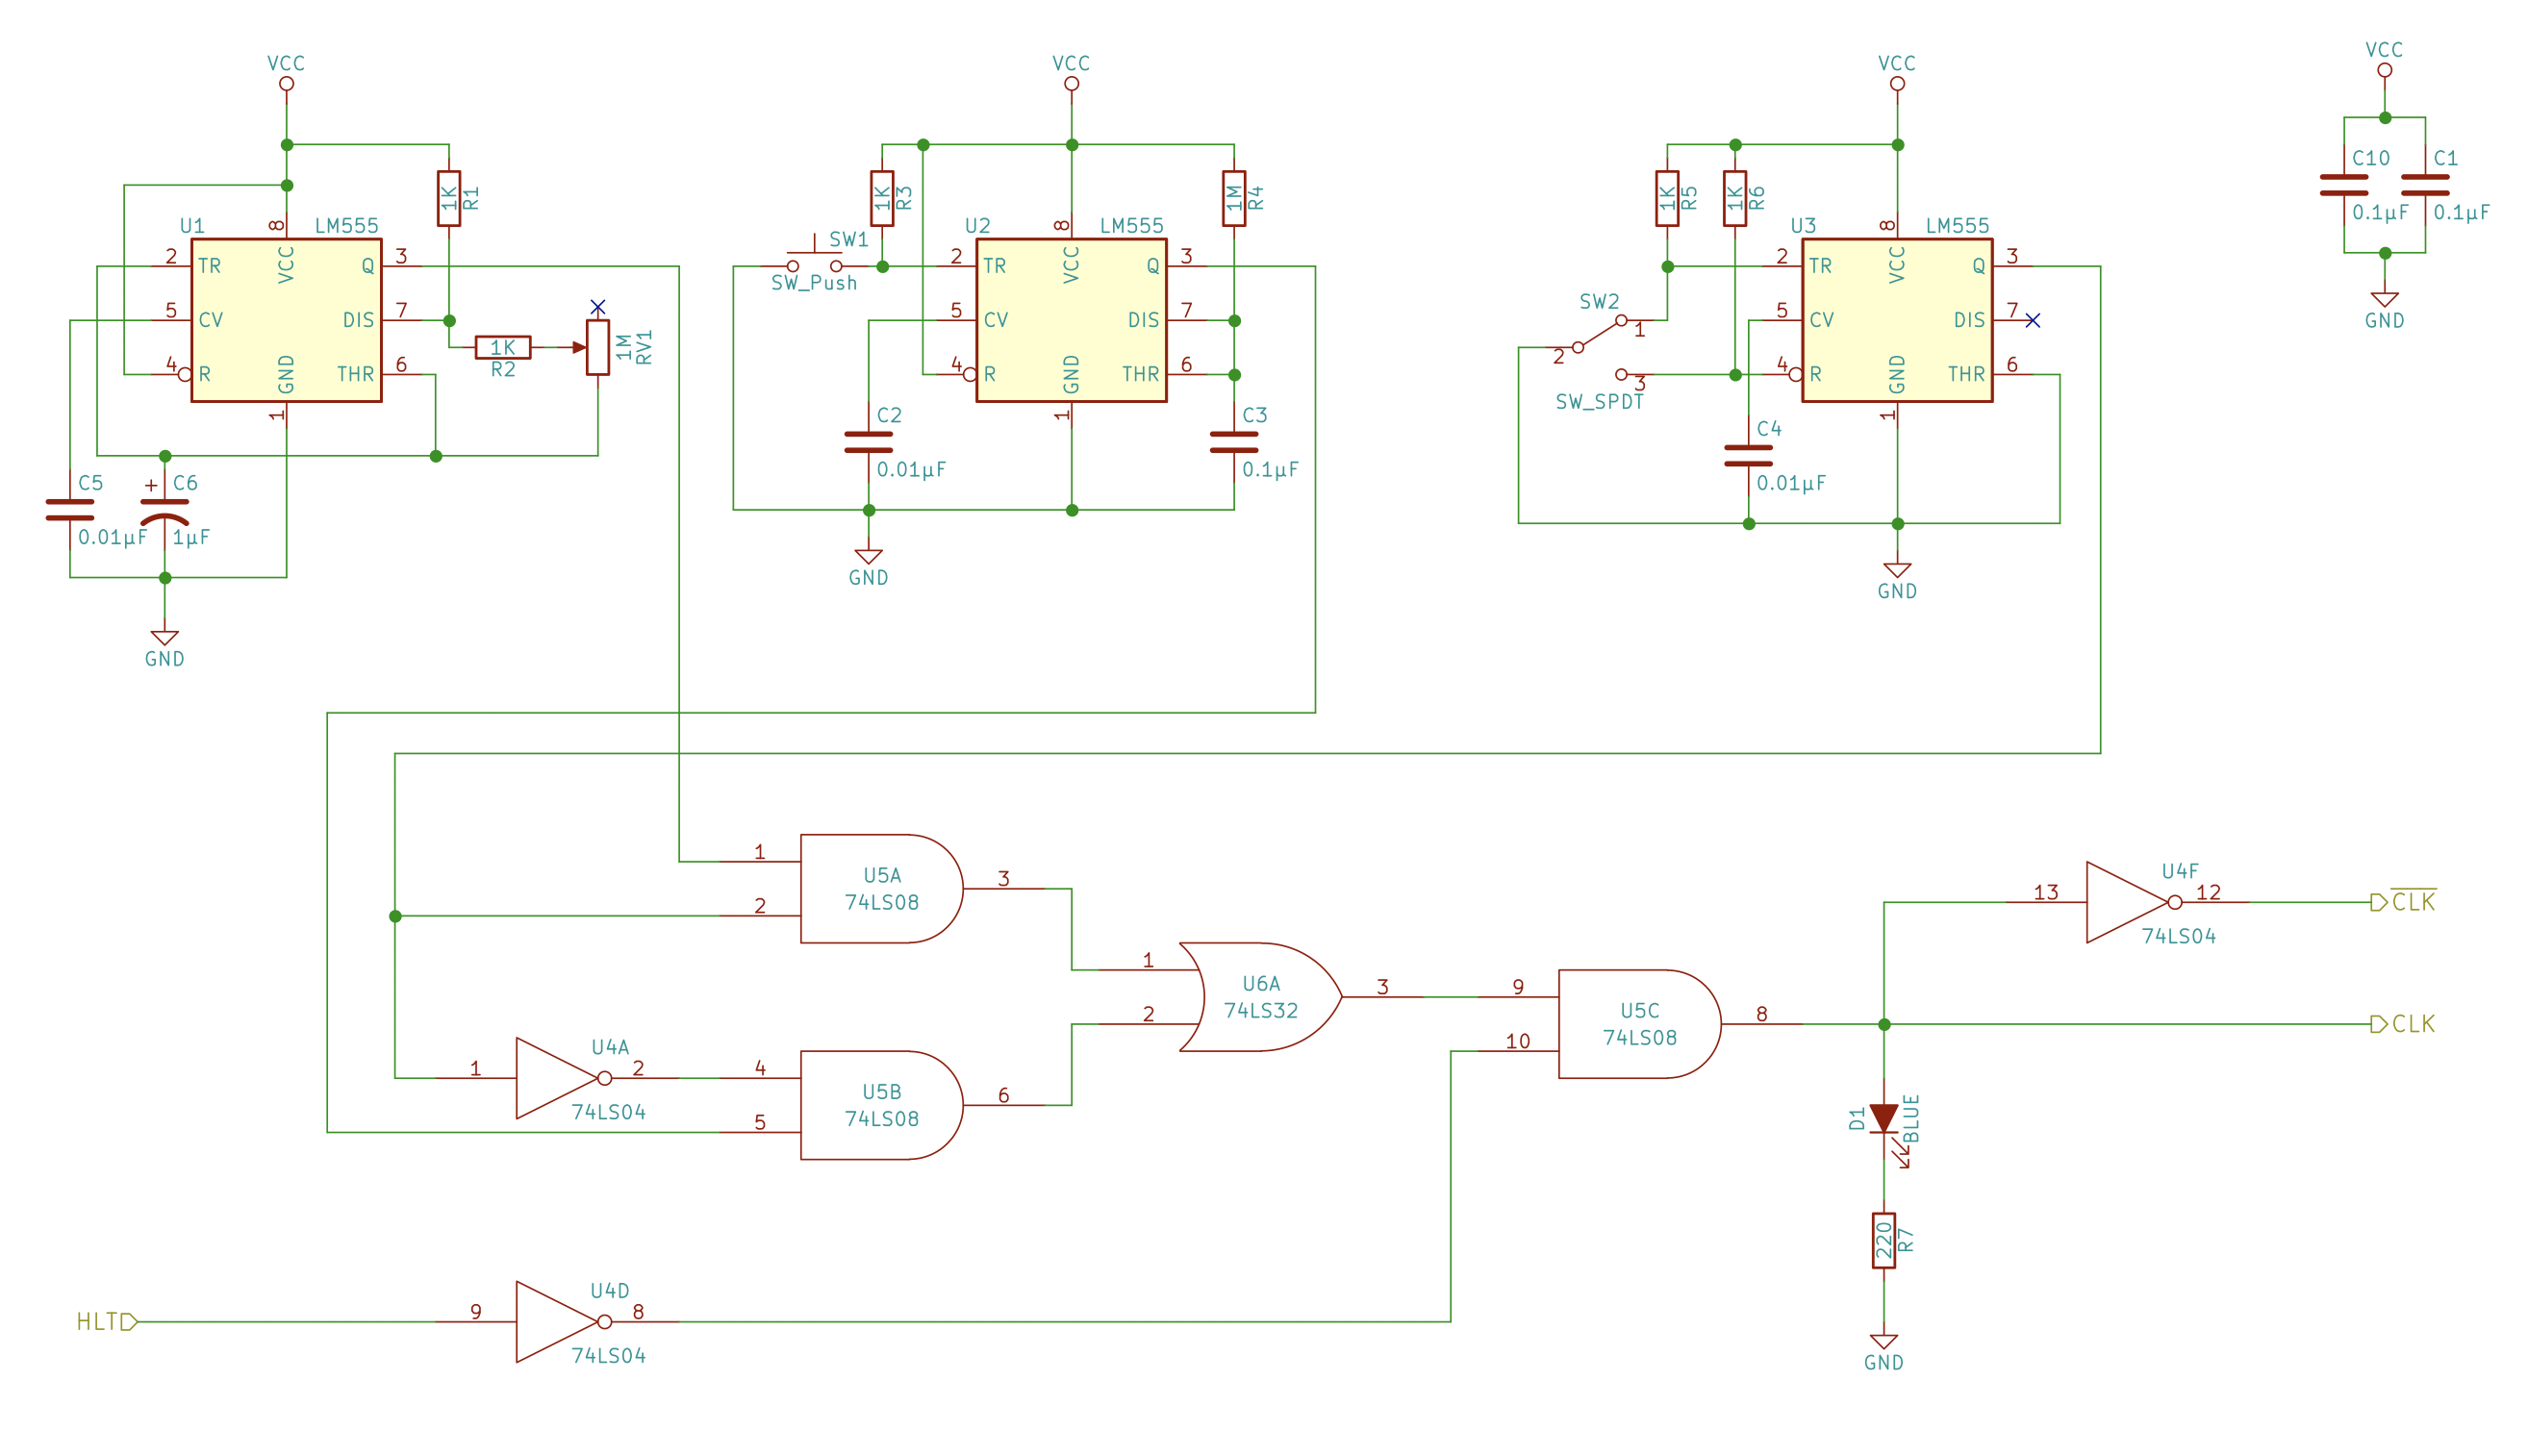
\includegraphics[width=0.7\textwidth]{schematics_clock.png}}
  \caption{\label{schematics_clock} Esquema do Clock} 
\end{figure}

\subsubsection{Registradores}
Assim, como o clock é essencial para o funcionamento do computador, os registradores também são, estes são como variáveis, mas em hardware. A maioria das CPUs possuem vários registradores que armazenam pequenas quantidades de dados. Em nossa CPU de breadboard, estão sendo desenvolvido três registradores de 8 bits: A, B e IR. Os registradores A e B são para uso geral – armazenamento de dados (de forma numérica). Já o IR (instruction register), apesar de funcionar da mesma forma, é usado para armazenar a instrução atual que está sendo executada, ou seja a instrução que foi chamada através da vibração mais recente do clock.

\vspace{1cm}
\begin{figure}[H] \centering 
  \makebox[\textwidth][c]{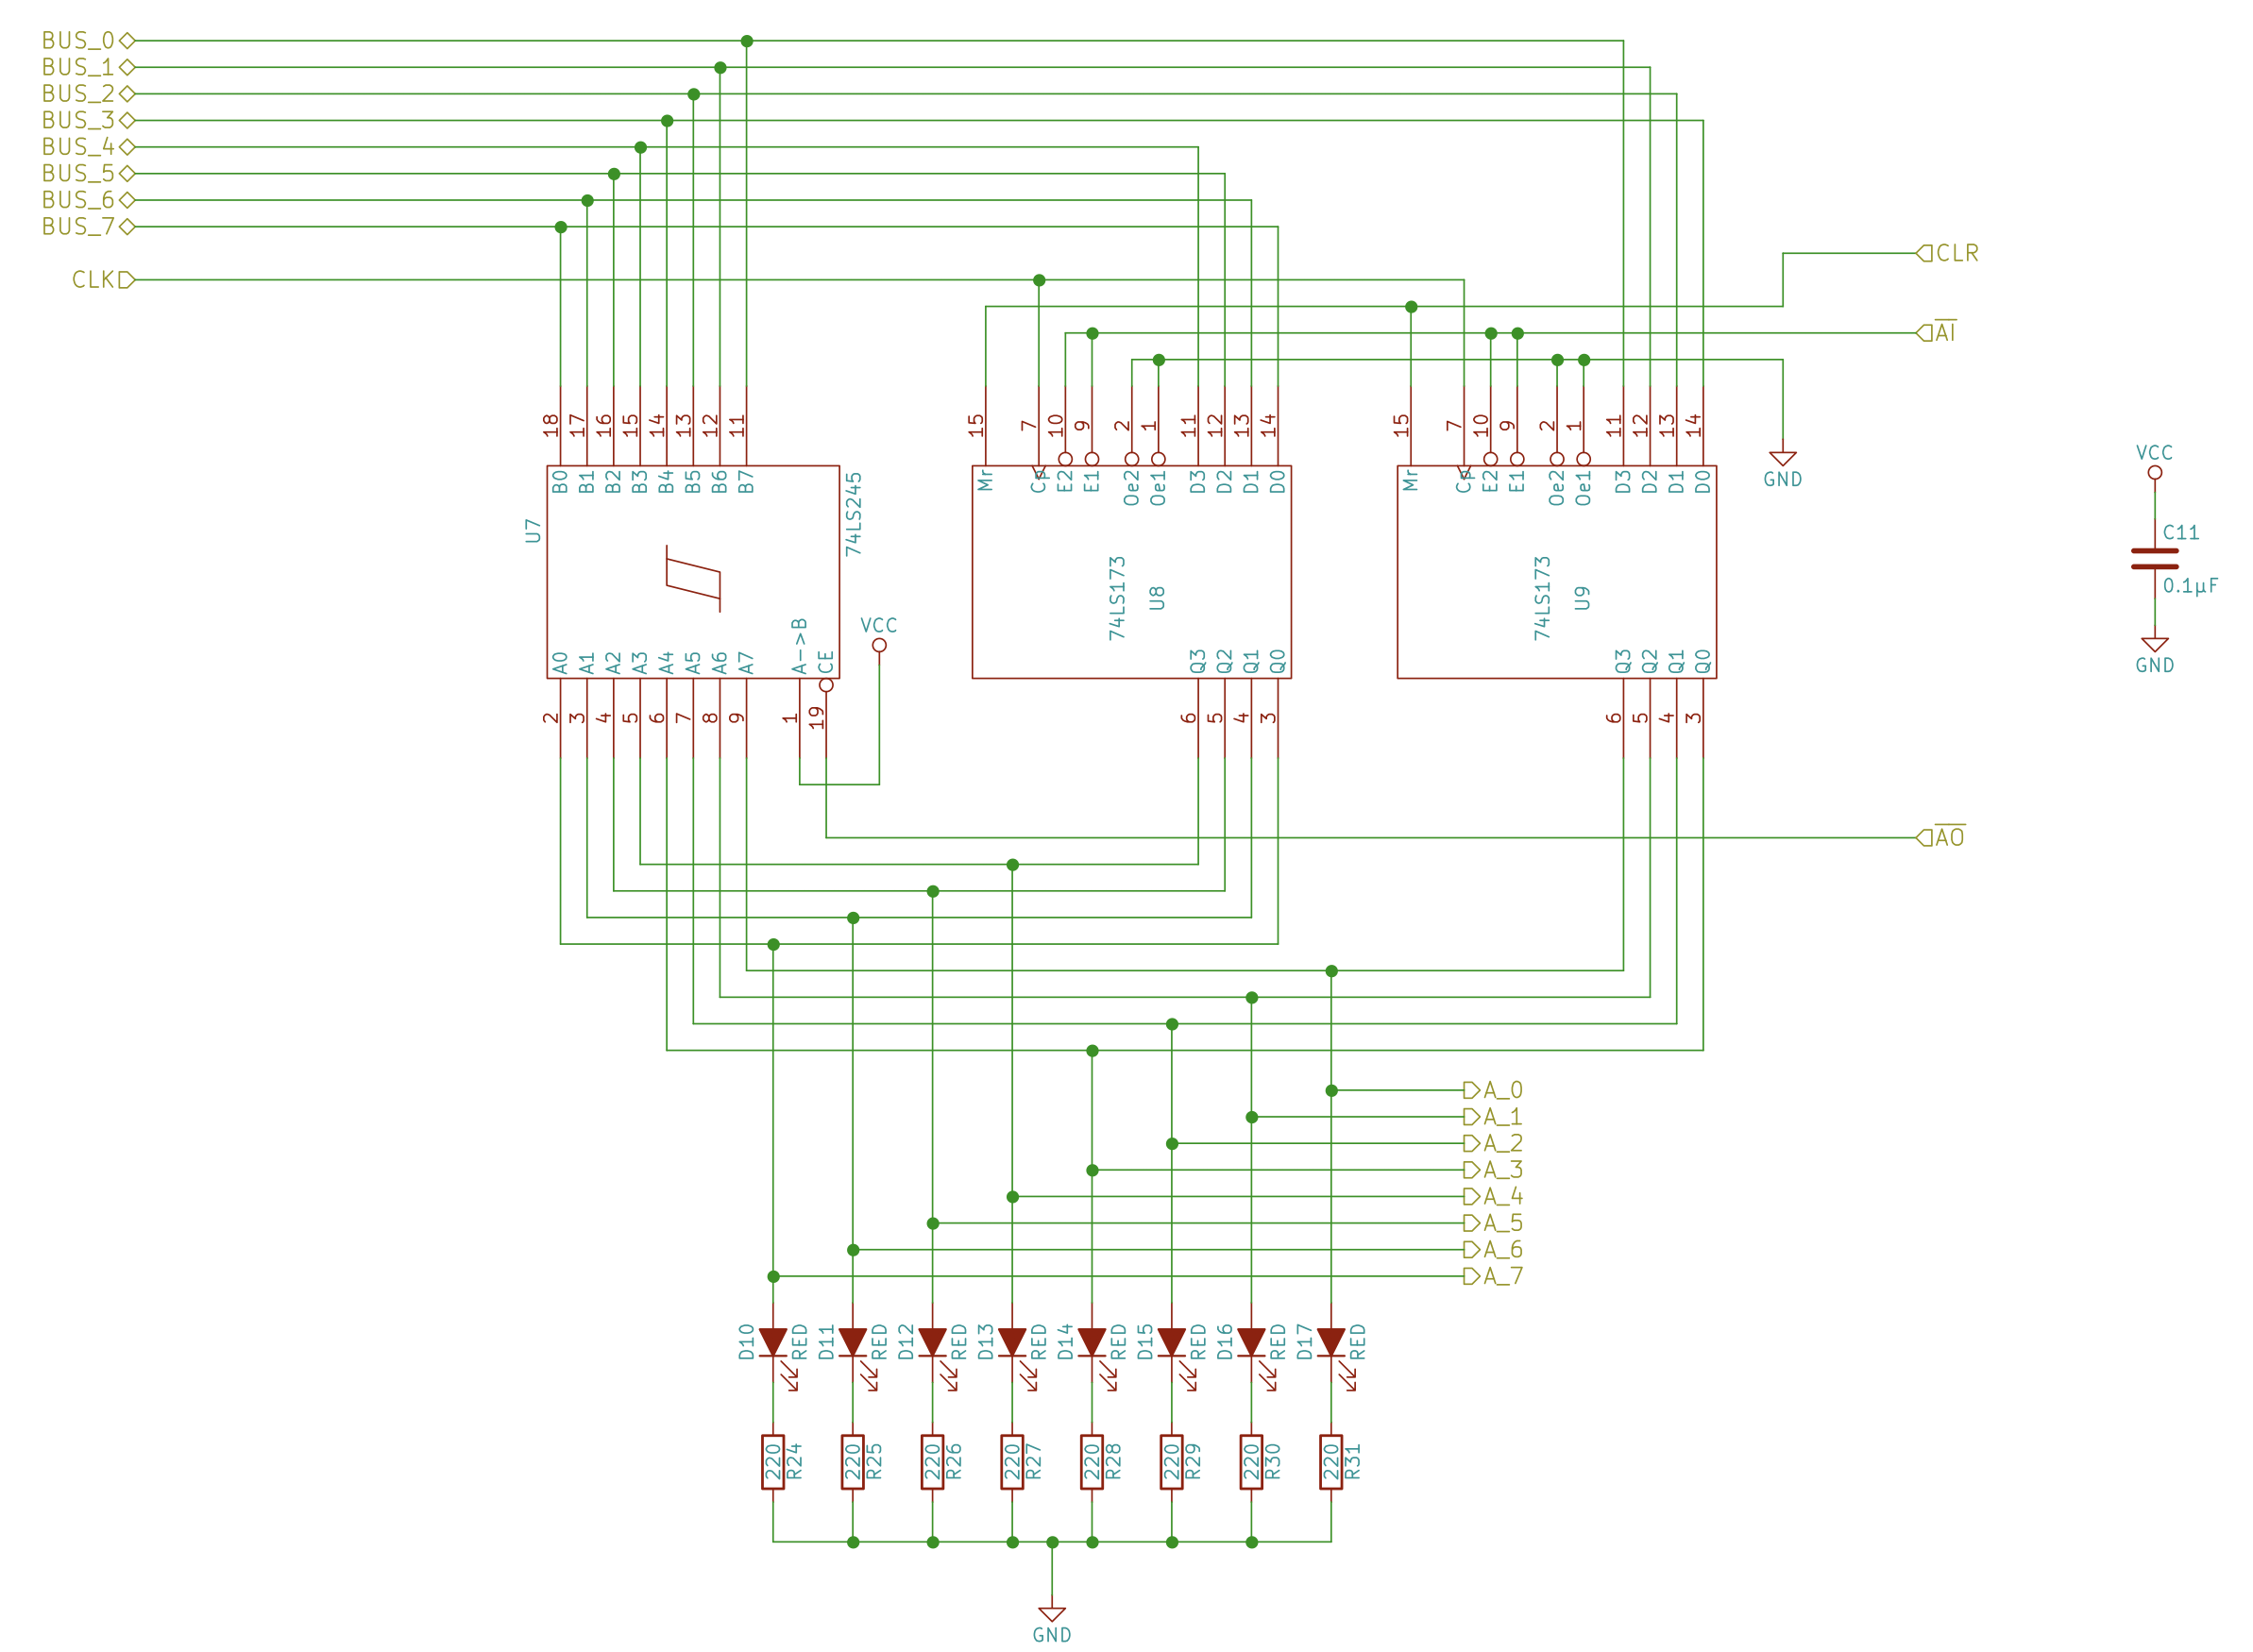
\includegraphics[width=0.7\textwidth]{schematics_a_register.png}}
  \caption{\label{schematics_a_register} Esquema do Registrador A} 
\end{figure}

\vspace{1cm}
\begin{figure}[H] \centering 
  \makebox[\textwidth][c]{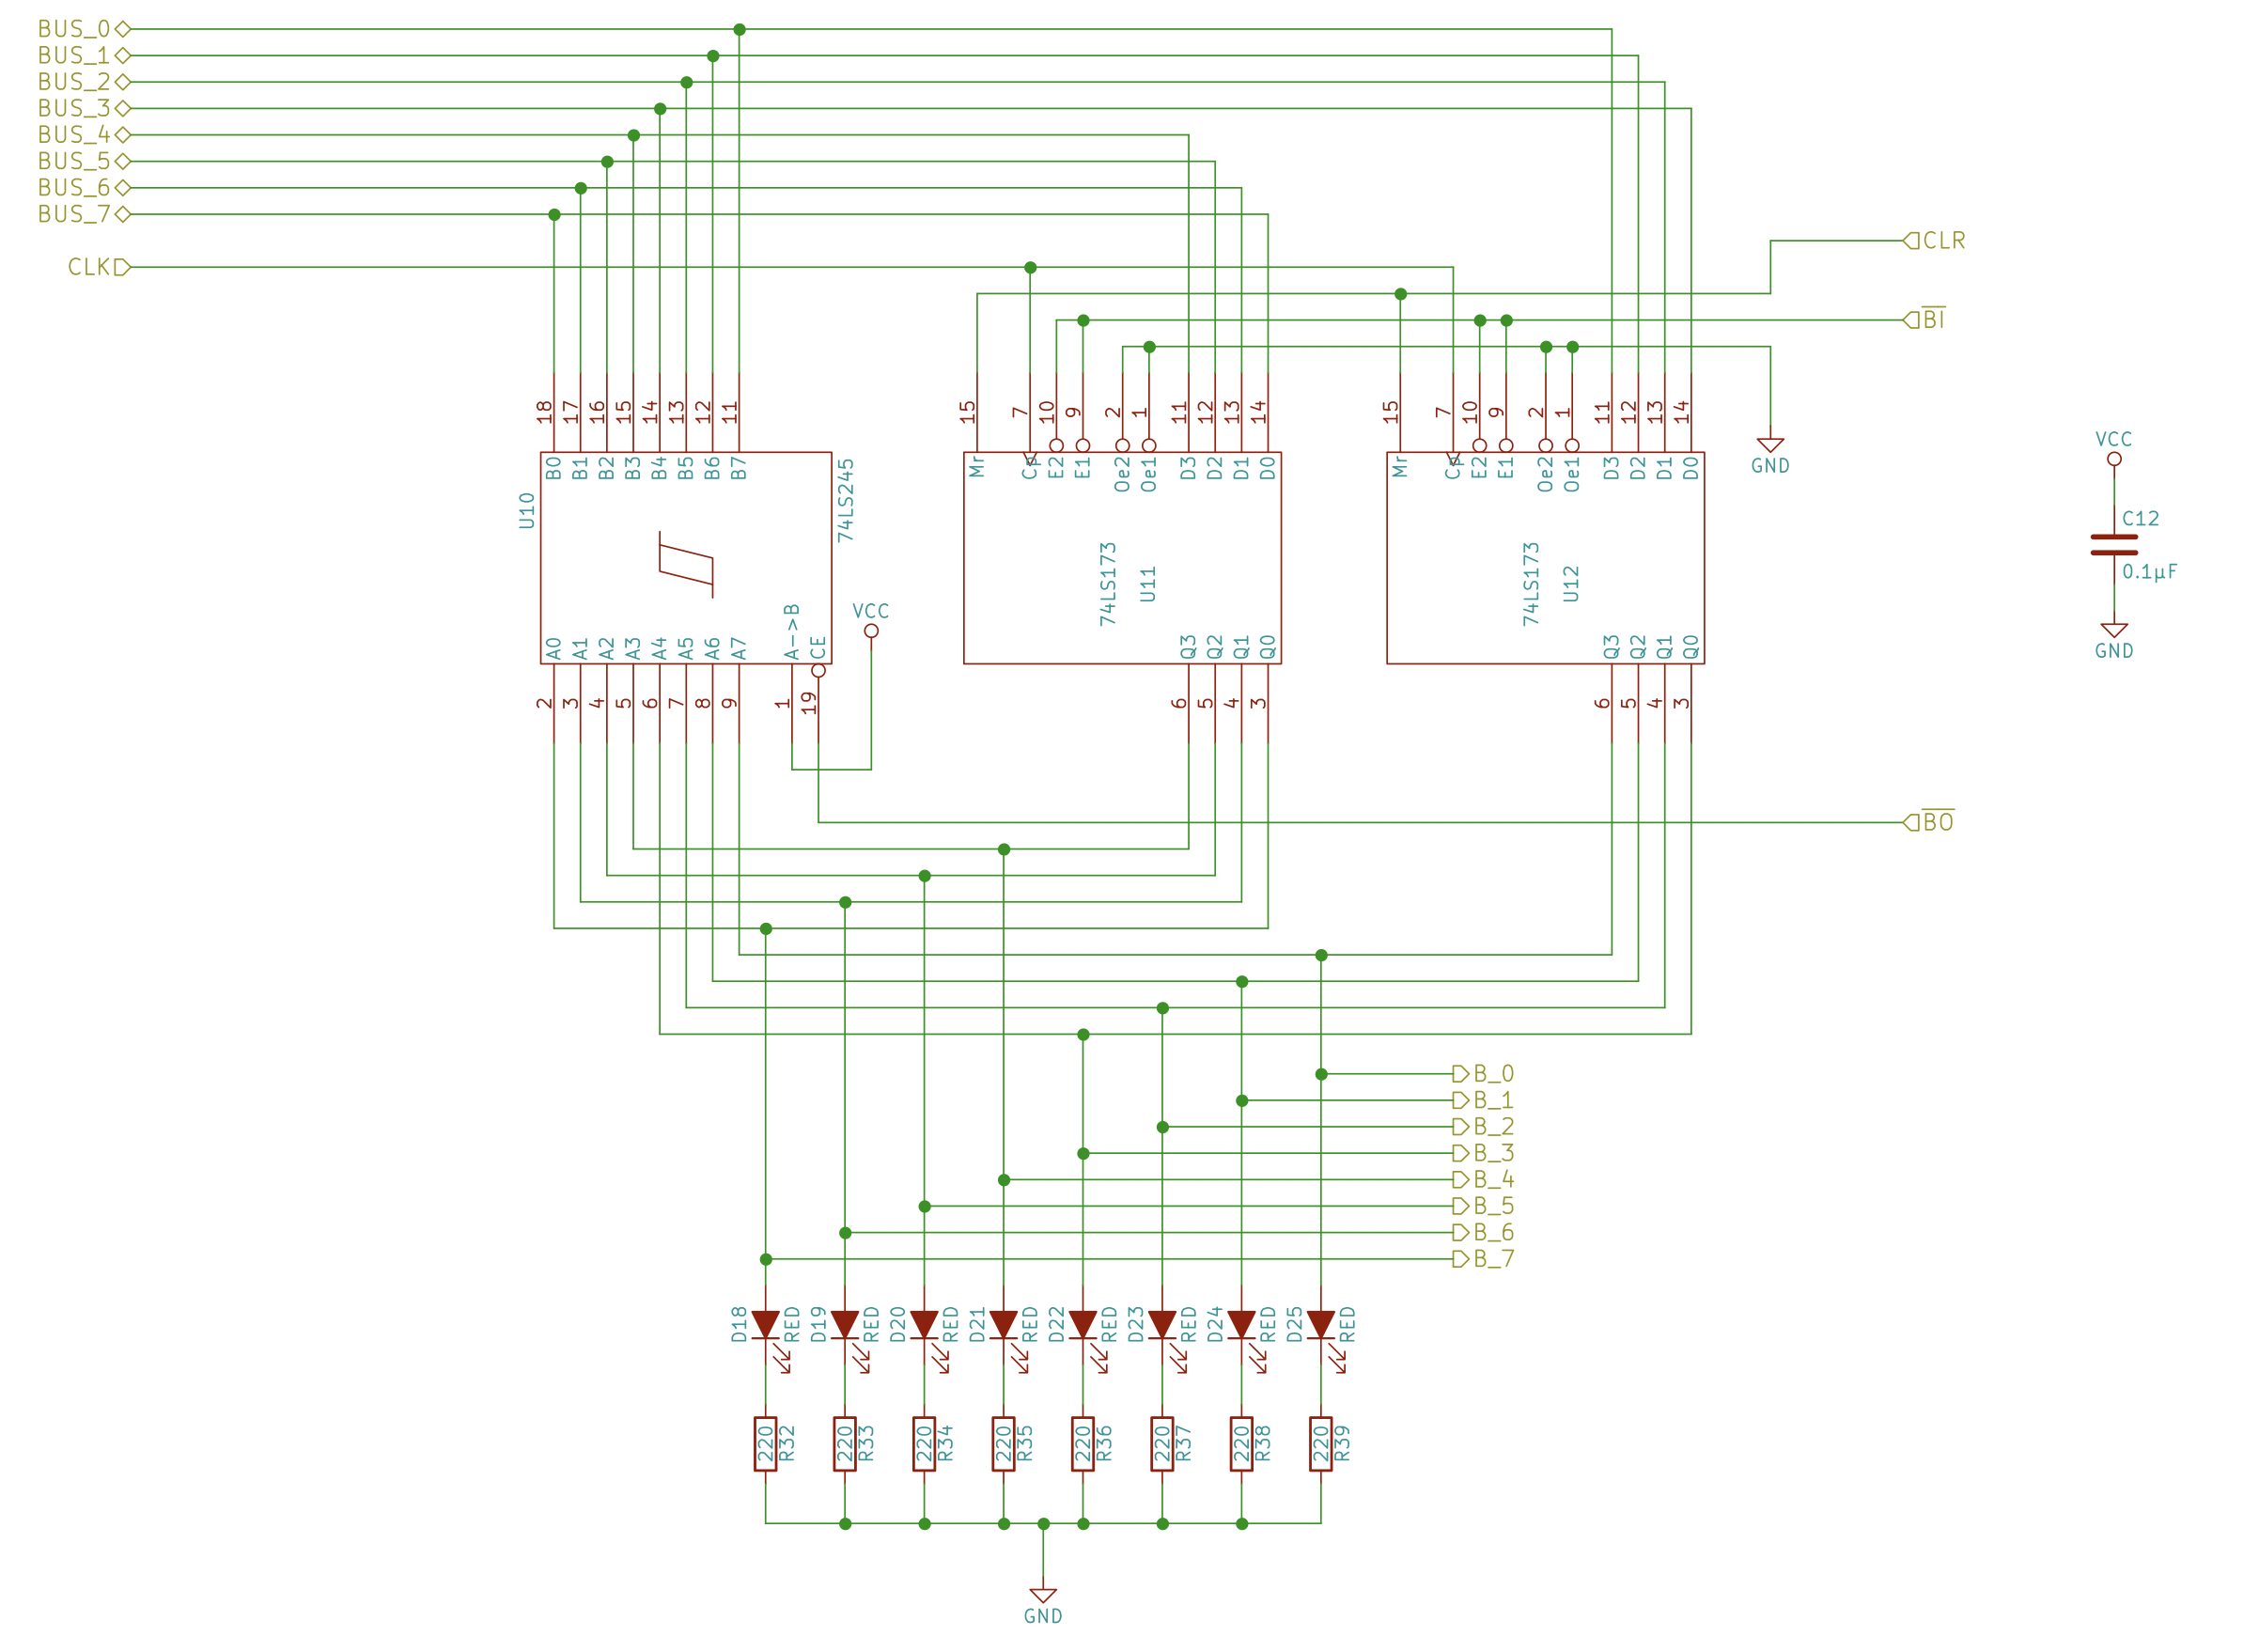
\includegraphics[width=0.7\textwidth]{schematics_b_register.png}}
  \caption{\label{schematics_b_register} Esquema do Registrador B} 
\end{figure}

\vspace{1cm}
\begin{figure}[H] \centering 
  \makebox[\textwidth][c]{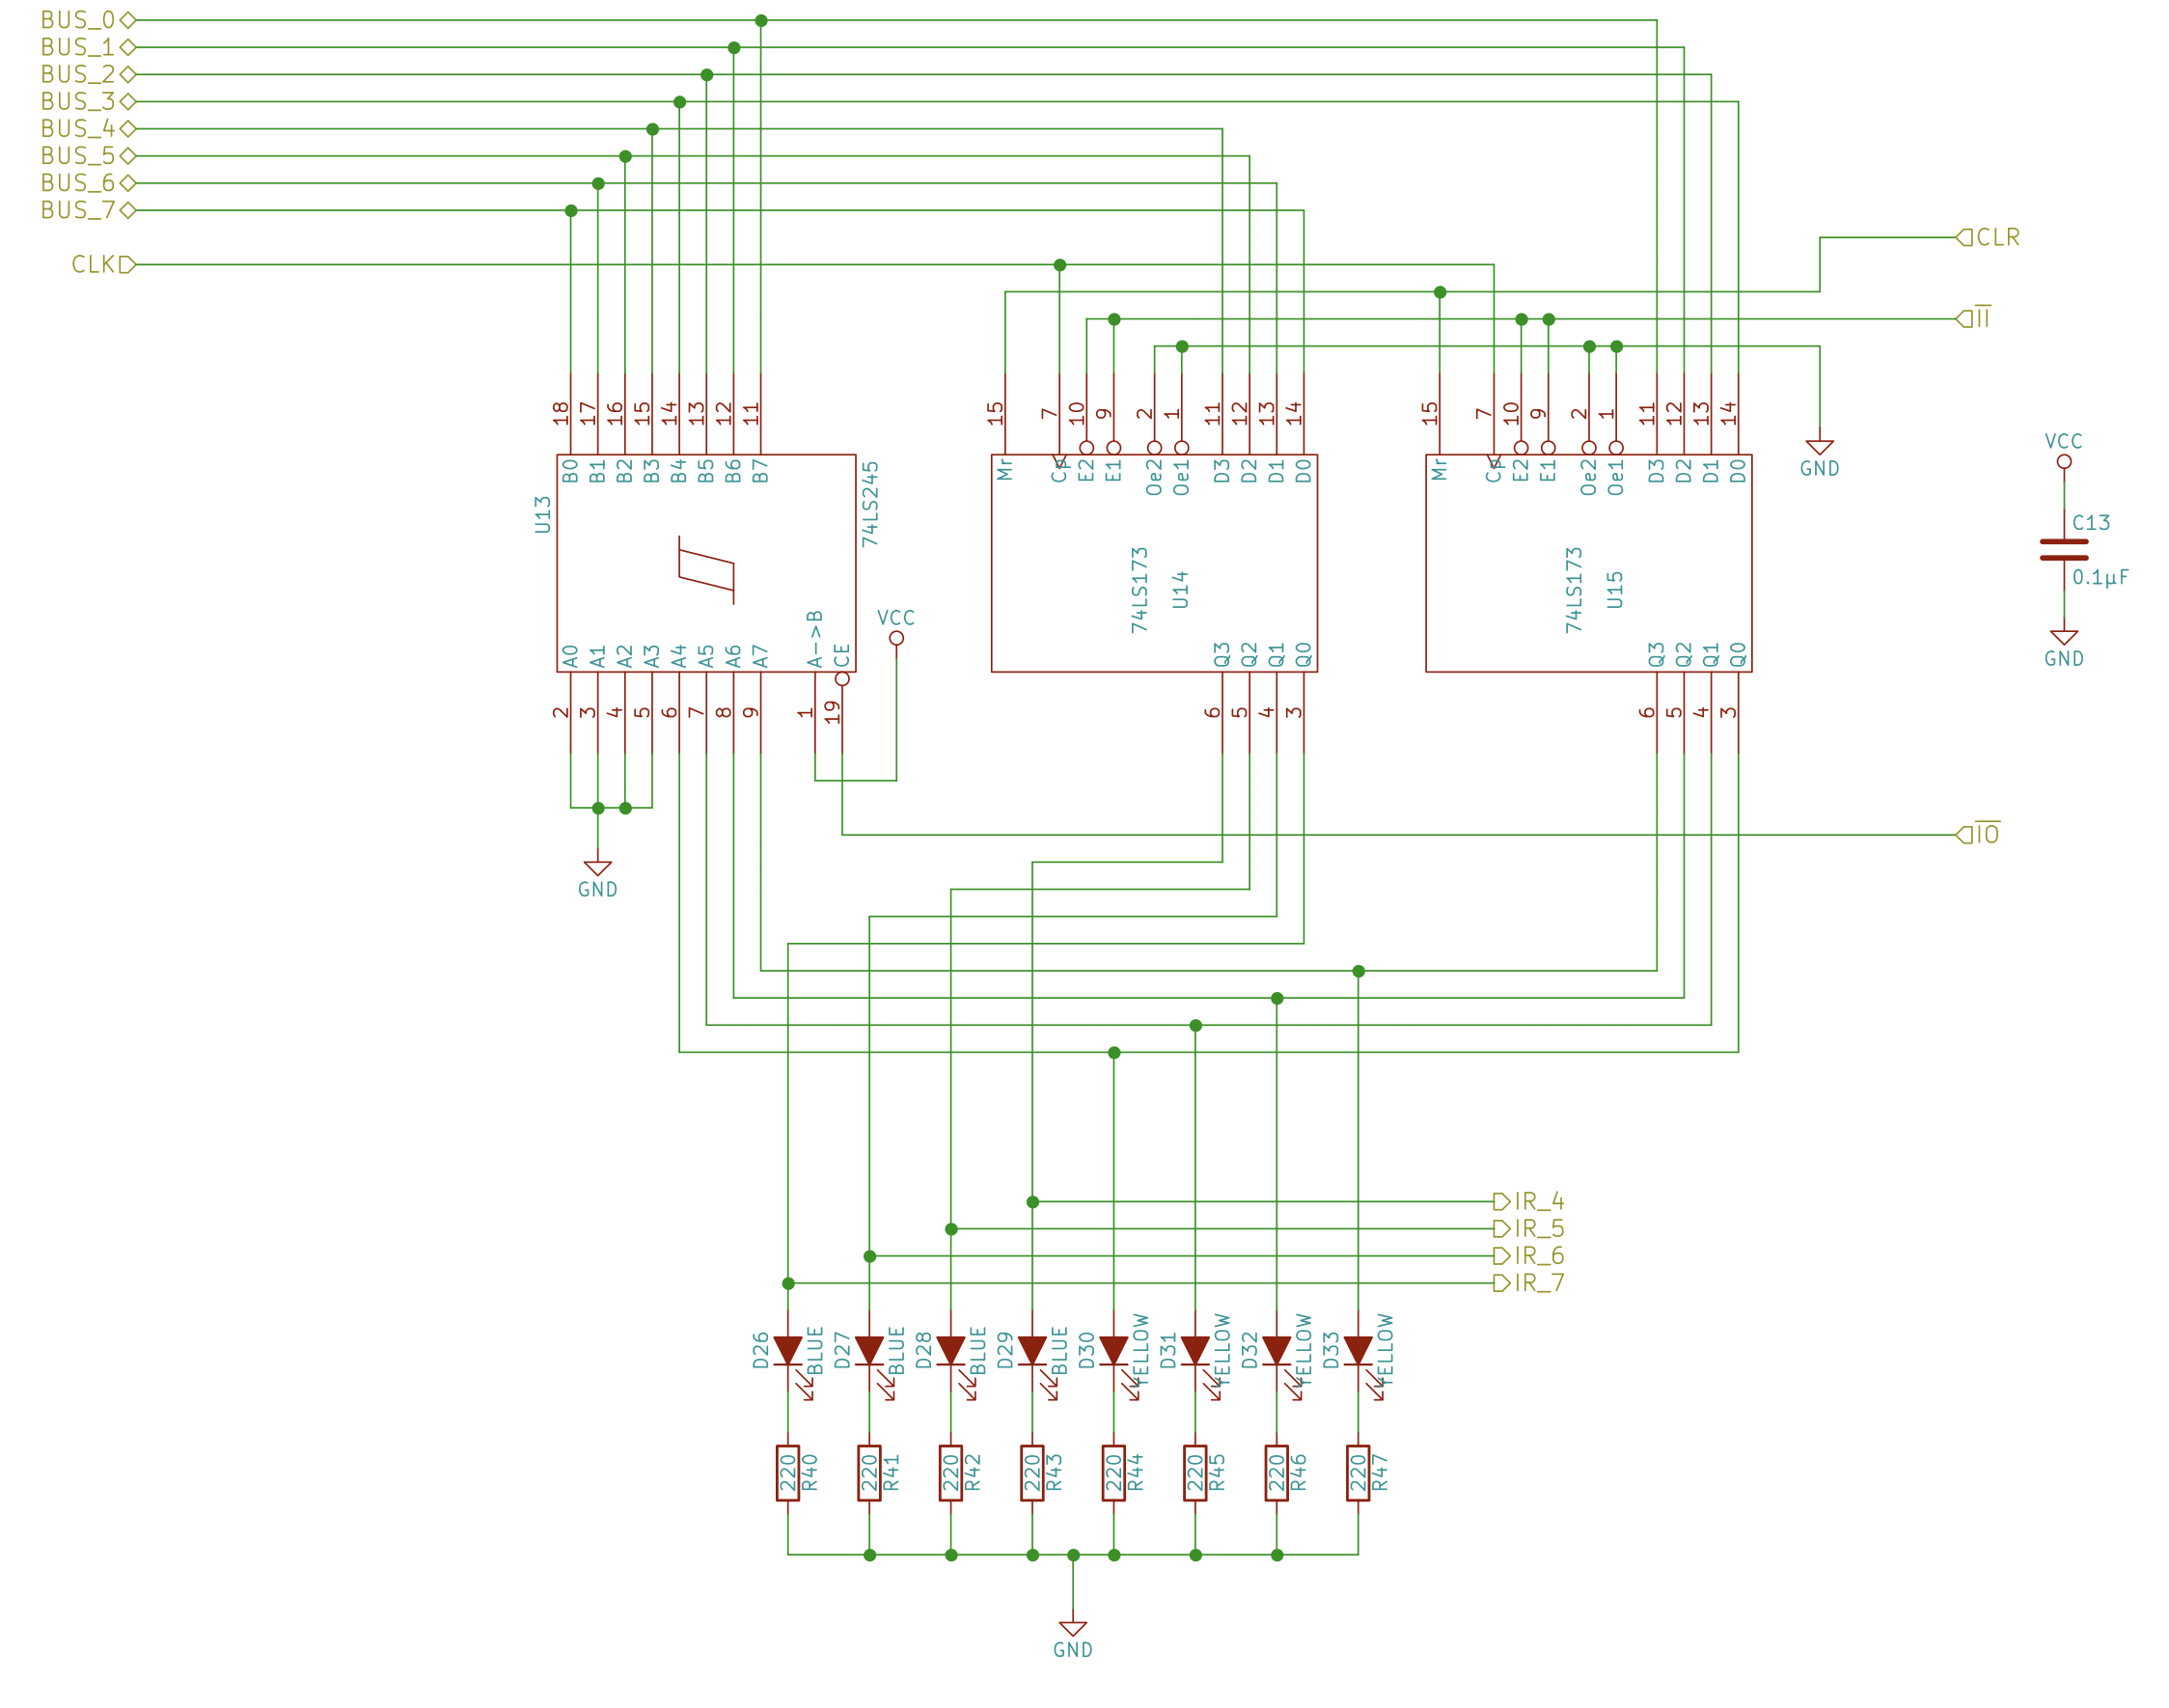
\includegraphics[width=0.7\textwidth]{schematics_ir.png}}
  \caption{\label{schematics_ir} Esquema do Registrador IR} 
\end{figure}

\subsubsection{Unidade Logica Aritmética  (ULA)}
Para o funcionamento de um computador, é preciso que dados sejam manipulados, assim chegamos ao modulo de lógica aritmética, conhecida como unidade lógica aritmética (ULA) de uma CPU, esta geralmente é capaz de executar várias operações aritméticas, bit a bit e de comparação em números binários. Em nossa CPU de breadboard, a ULA pode apenas adicionar e subtrair, a final essa implementação é apenas para fins acadêmicos e não tem a necessidade de ser performática em termos de eficiência computacional. Ele é conectada aos registradores A e B sendo capaz de gerar a soma de A + B ou a diferença de A-B.

\vspace{1cm}
\begin{figure}[H] \centering 
  \makebox[\textwidth][c]{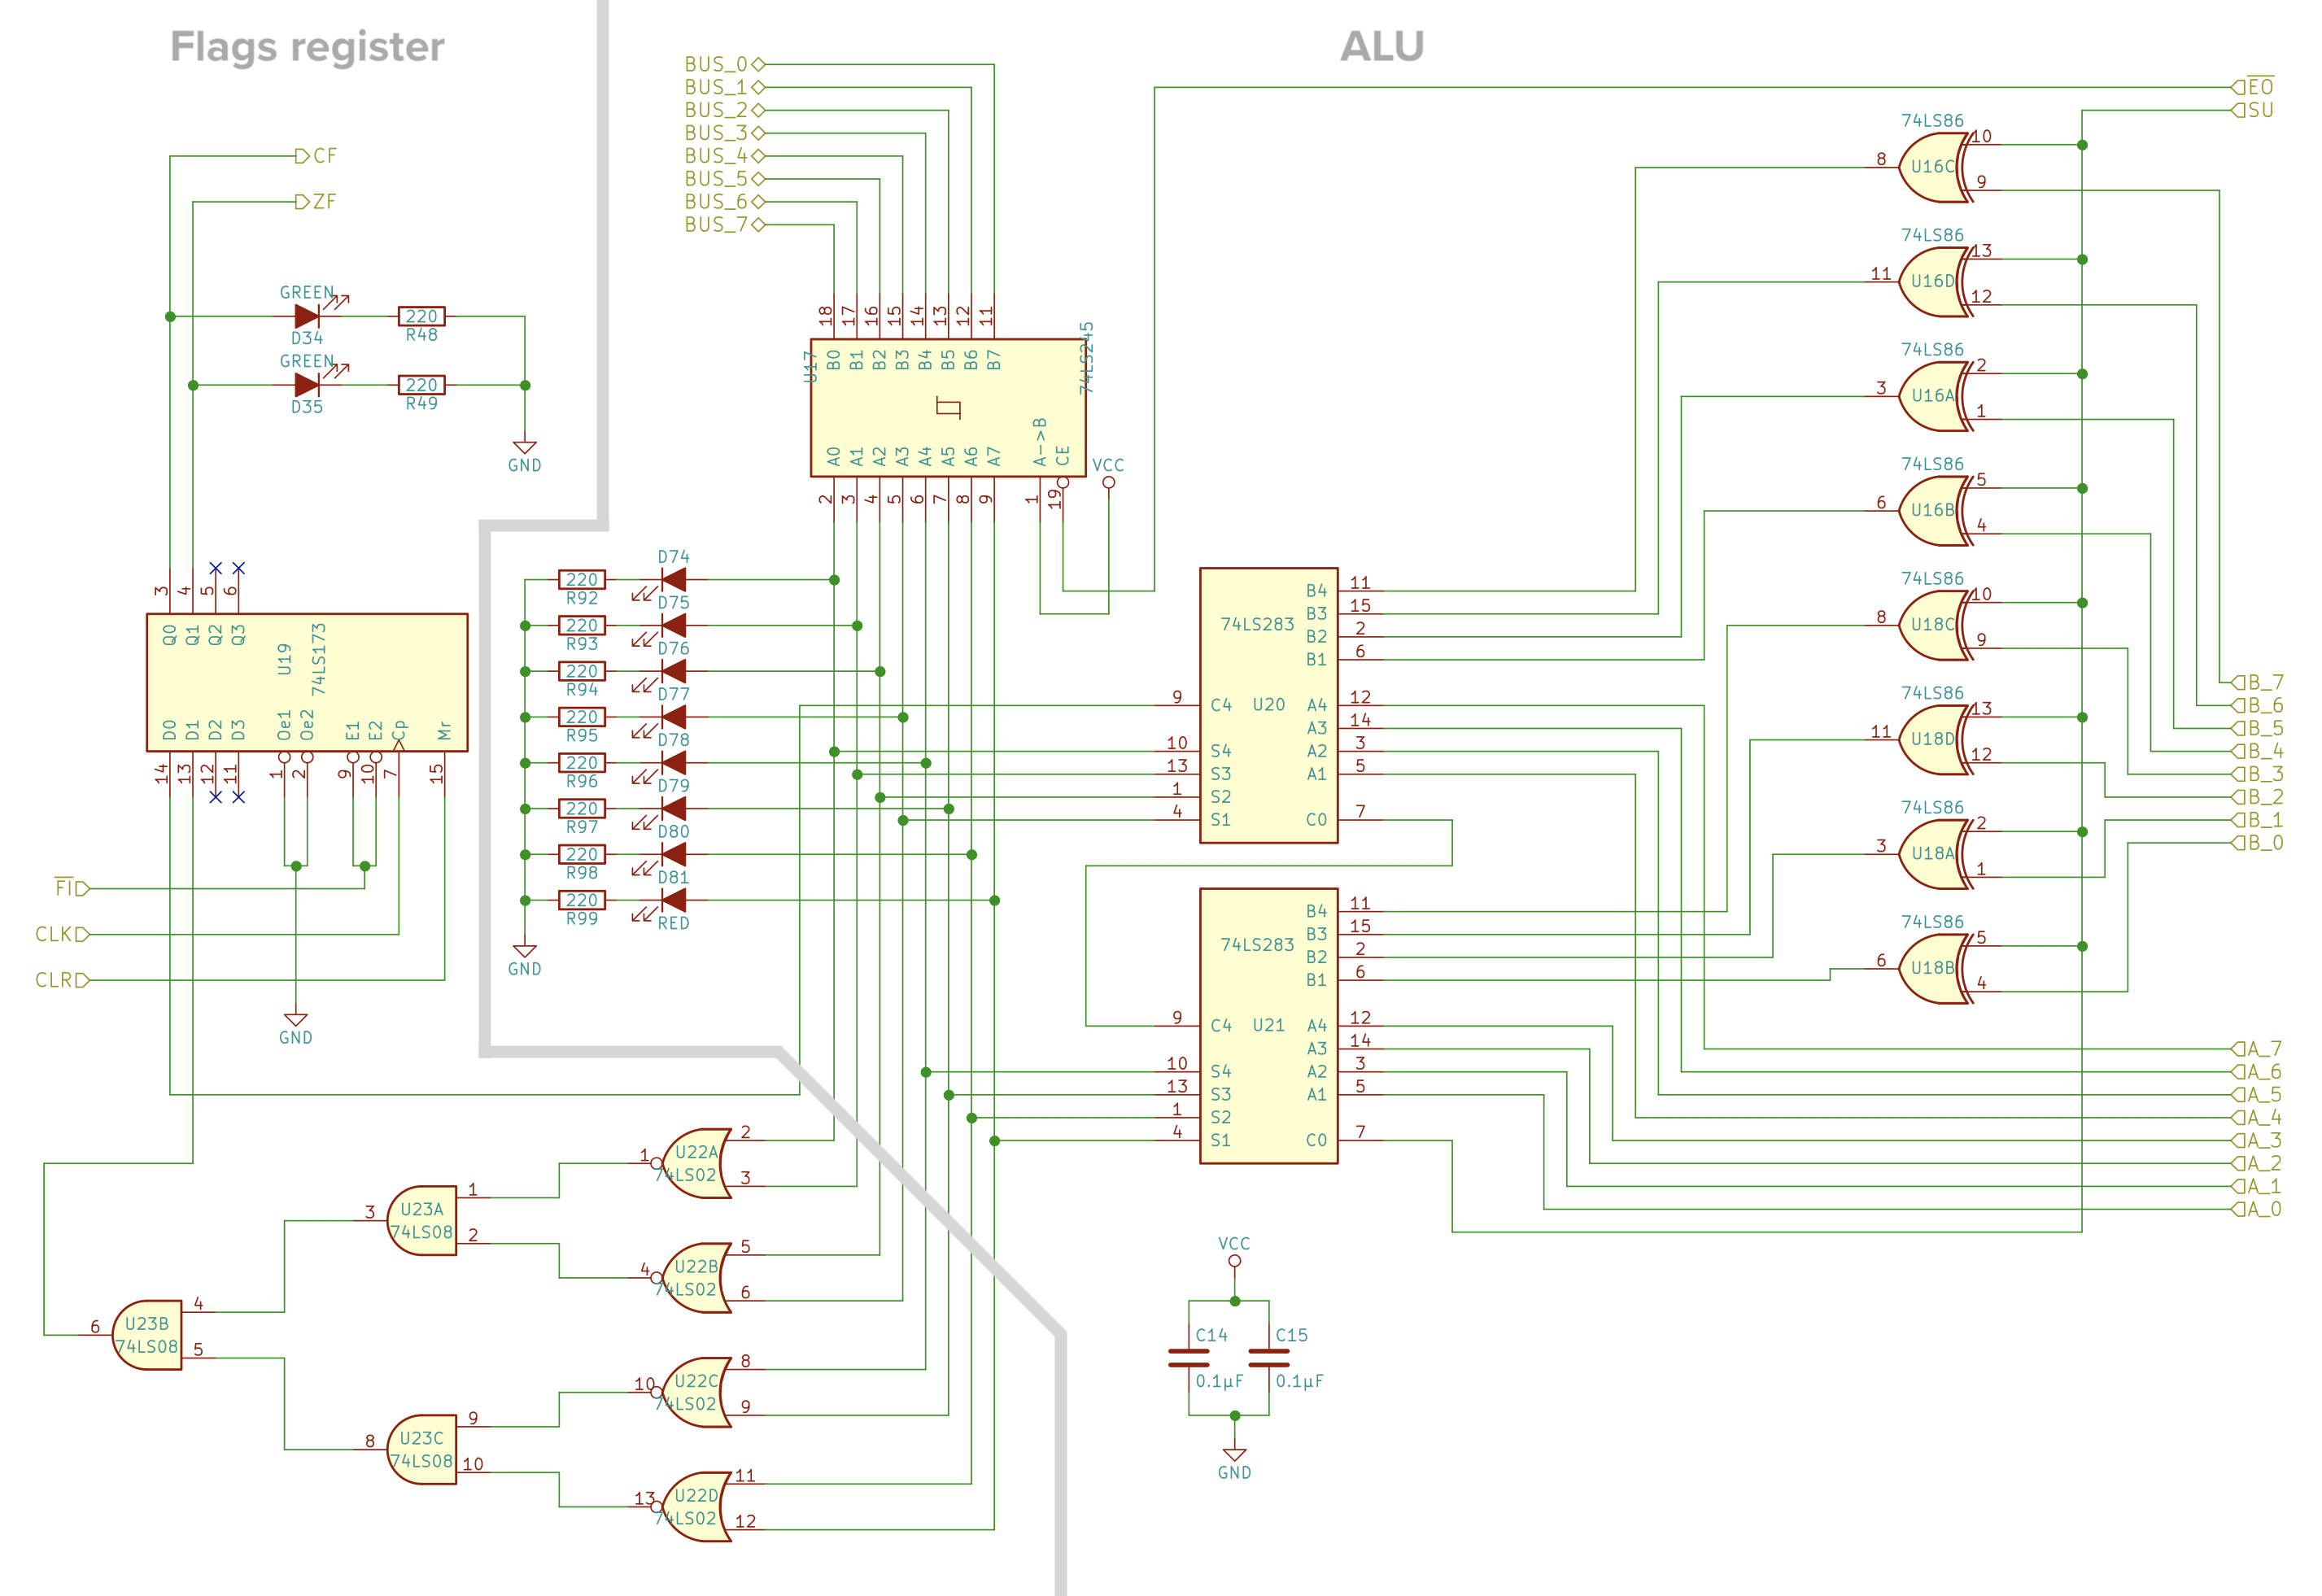
\includegraphics[width=0.7\textwidth]{schematics_alu.png}}
  \caption{\label{schematics_alu} Esquema da ULA} 
\end{figure}

\subsubsection{Memoria (RAM)}
Computadores em geral tem 2 memorias, o HD ou SSD e a memoria RAM, o HD (Hard Drive) e SSD (Solid State Drive) tem com objetivo armazenar dados de forma permanente, armazenam os dados em um espaço físico onde seu acesso é mais lento, porem, mesmo com o computador desligado os dados são guardados serão confiáveis após o computador ser religado. Já a memória de acesso aleatório, RAM, é uma memoria eletróncia e armazena dados apenas se o computador estiver ligado, porem consegue acessa-los de forma significativamente mais rápida. Um dos objetivos principais dessa memoria é armazenar o programa que o computador está executando no exato momento, bem como todos os dados que o programa precisa. Para o computador de breadboard que esta sendo desenvolvido, a memoria RAM utiliza endereços de 4 bits, o que significa que ele terá apenas 16 bytes de RAM, limitando o tamanho e a complexidade dos programas que poderão ser executados.

\vspace{1cm}
\begin{figure}[H] \centering 
  \makebox[\textwidth][c]{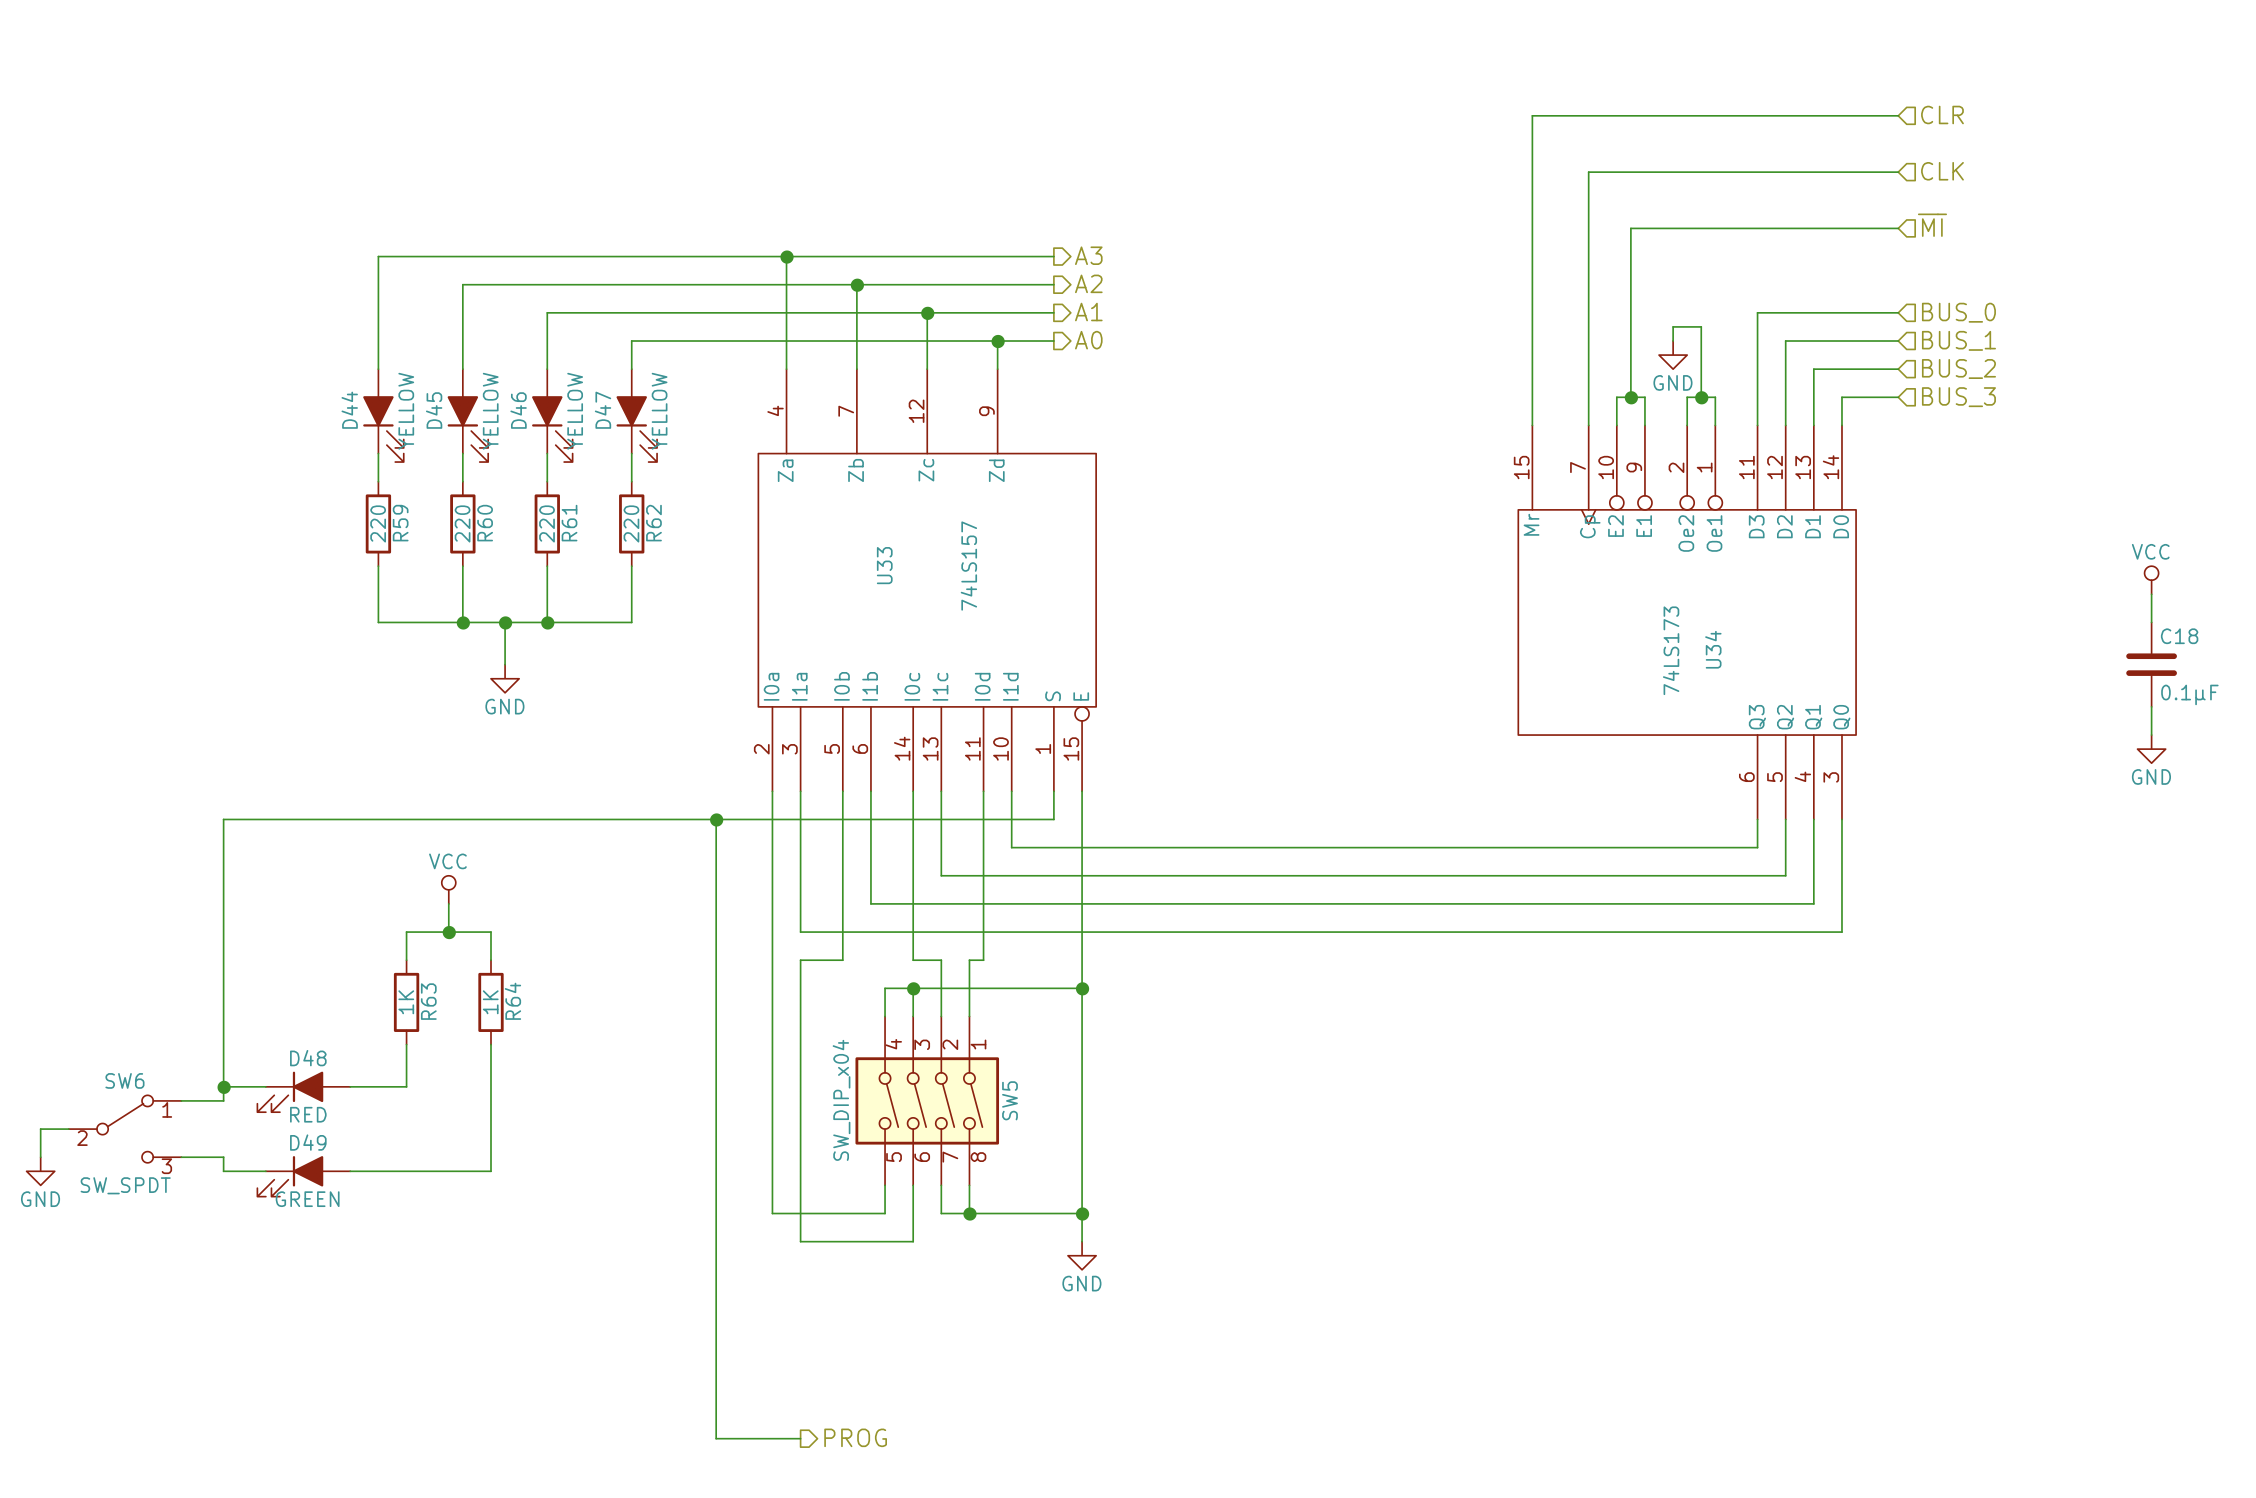
\includegraphics[width=0.7\textwidth]{schematics_mar.png}}
  \caption{\label{schematics_mar} Esquema da MAR} 
\end{figure}

\vspace{1cm}
\begin{figure}[H] \centering 
  \makebox[\textwidth][c]{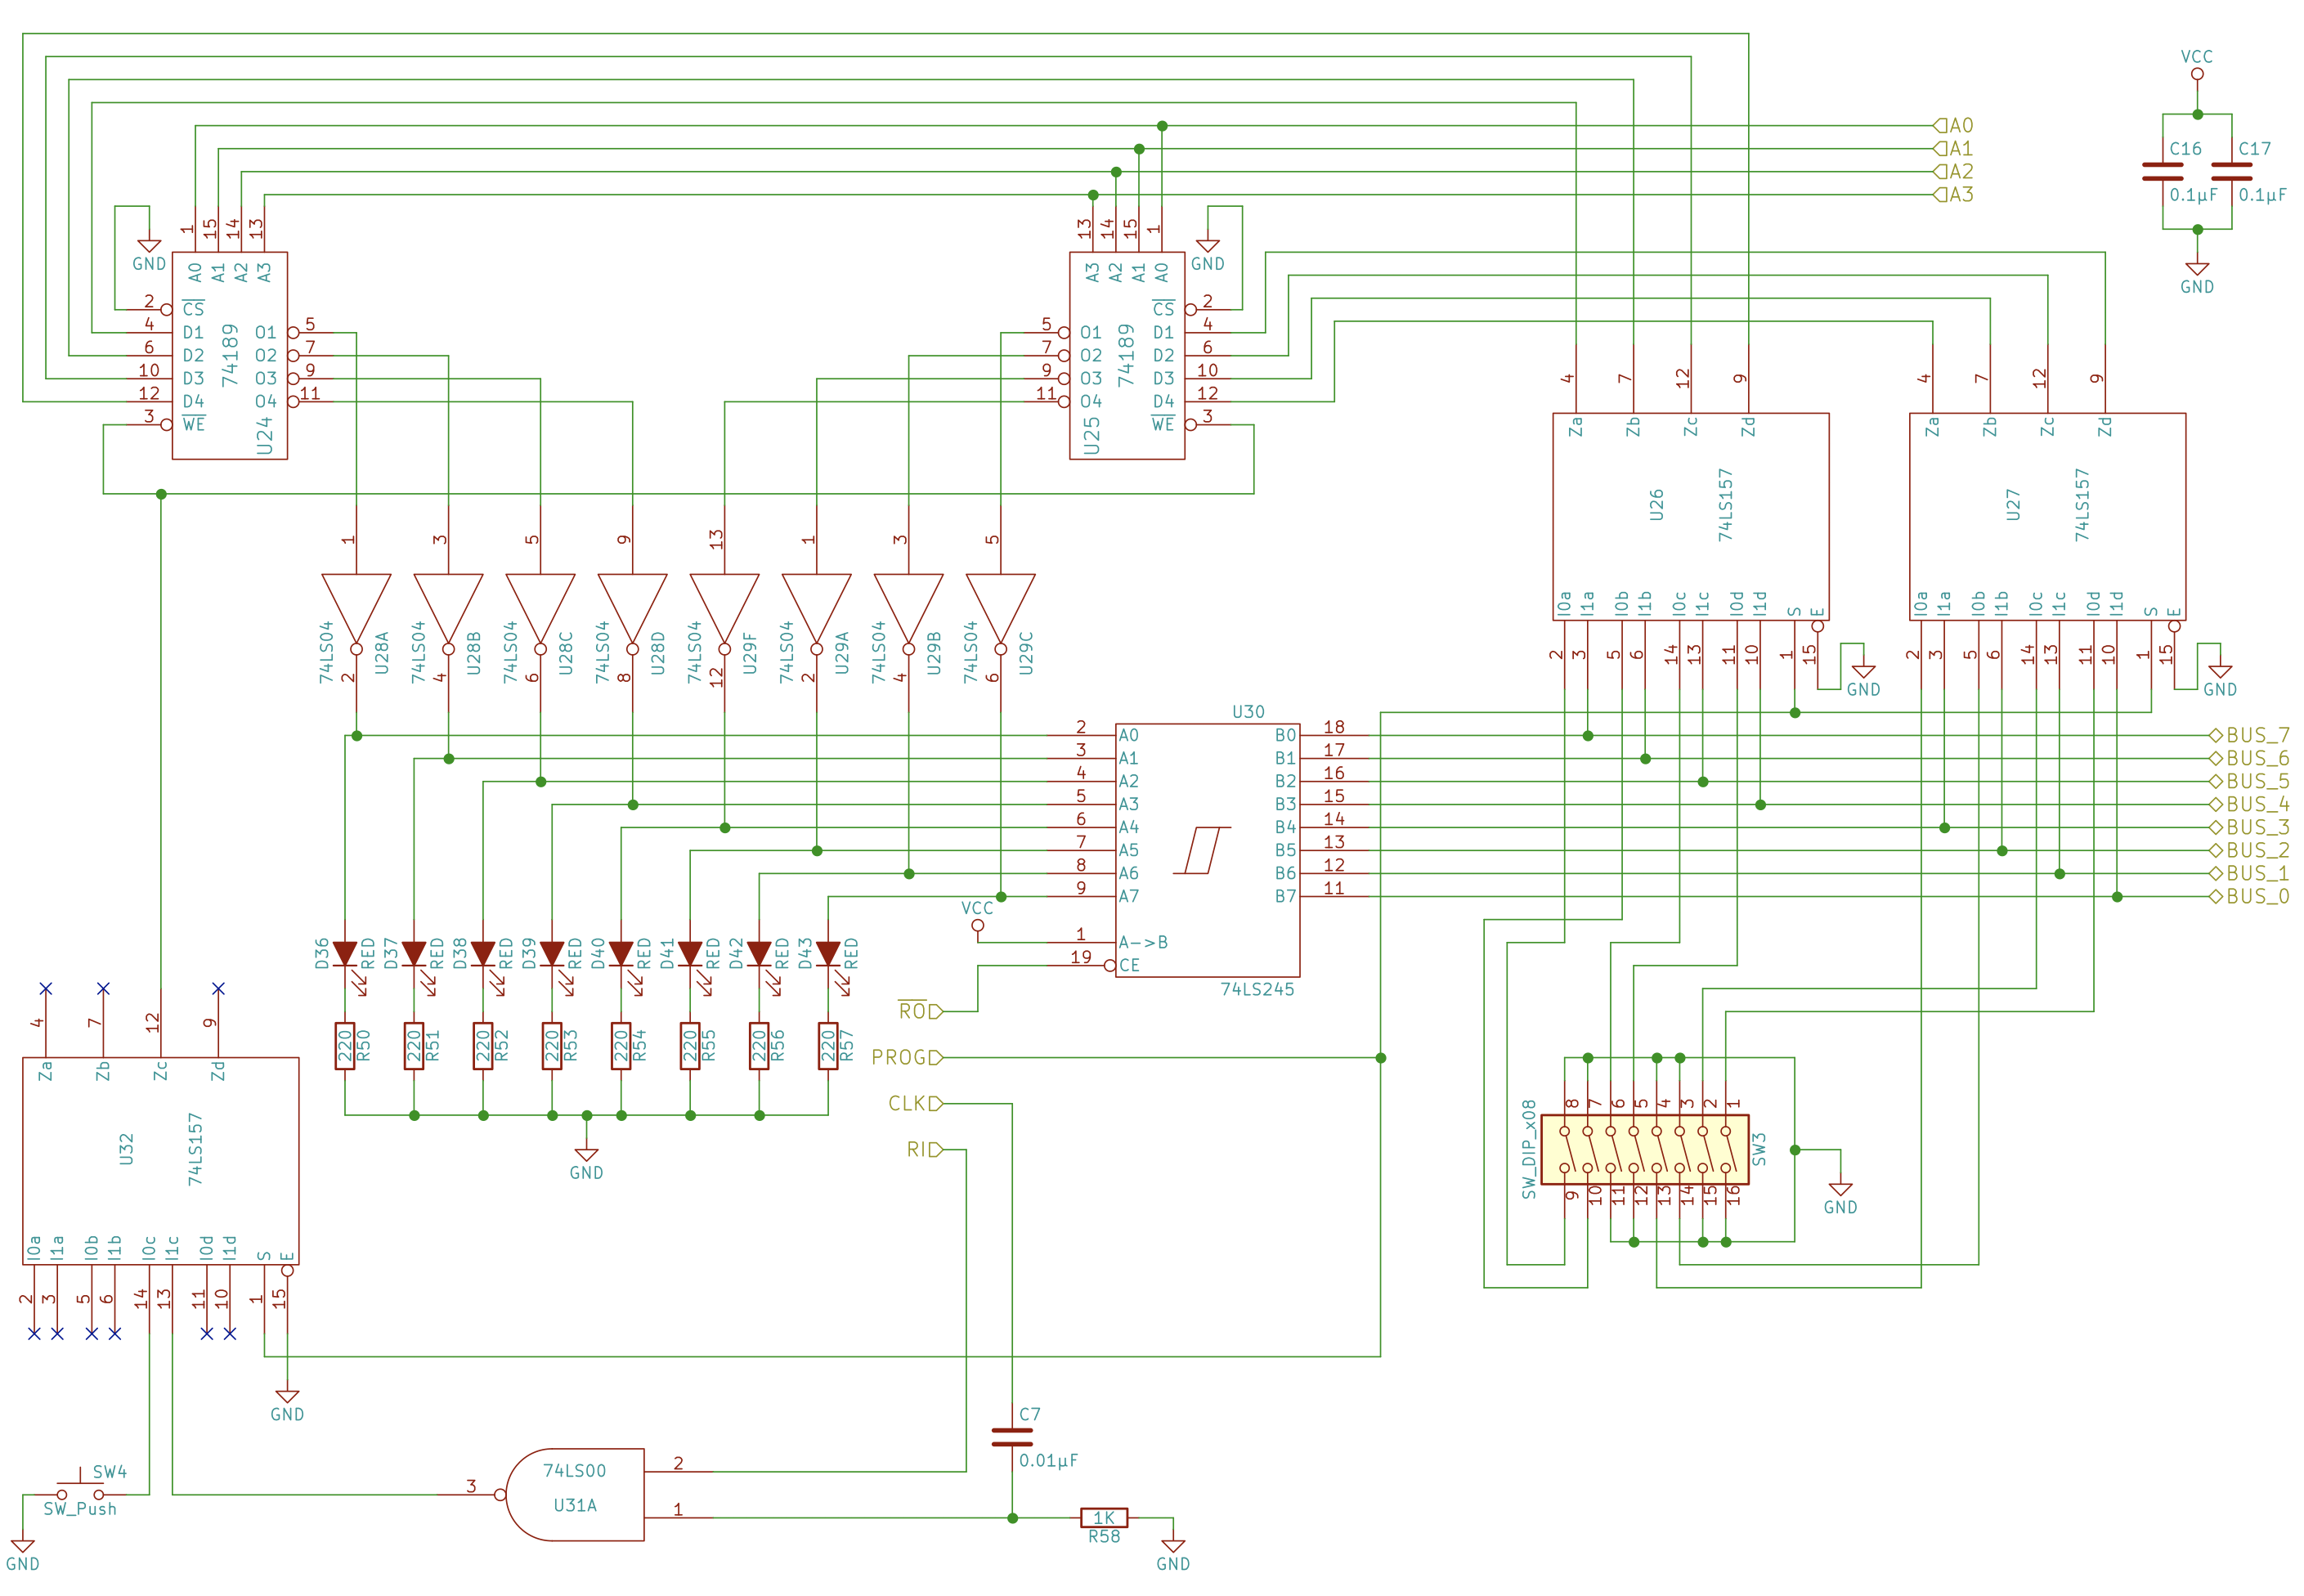
\includegraphics[width=0.7\textwidth]{schematics_ram.png}}
  \caption{\label{schematics_ram} Esquema da RAM} 
\end{figure}

\subsubsection{Contador}
O contador do programa (Program counter) conta em binário para acompanhar a instrução que o computador está executando no momento.

\vspace{1cm}
\begin{figure}[H] \centering 
  \makebox[\textwidth][c]{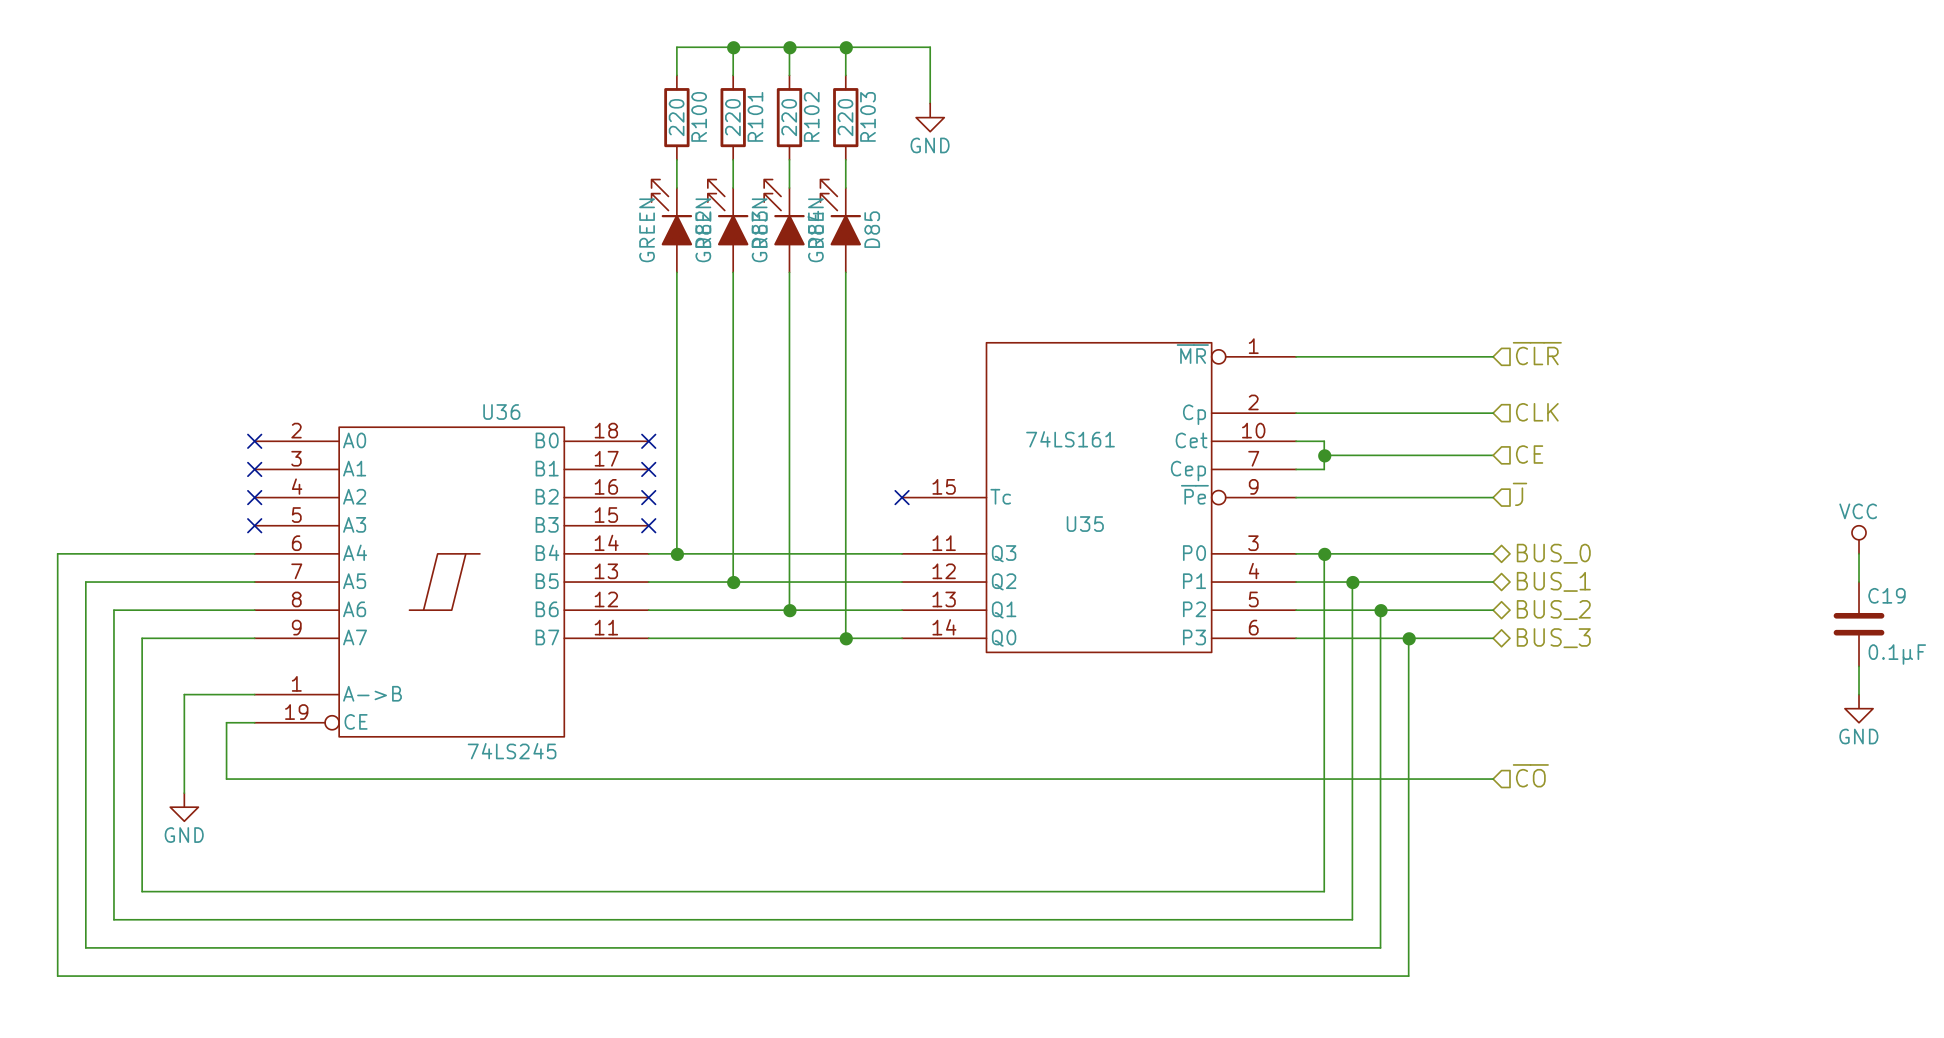
\includegraphics[width=0.7\textwidth]{schematics_pc.png}}
  \caption{\label{schematics_pc} Esquema do Contador} 
\end{figure}

\subsubsection{Registrador de Output}
O registrador de saída é um registrador especial para esse computador pois como não temos acesso a um monitor, este possibilita a leitura de dados de forma fácil e comum para seu usuário.  Este é semelhante a qualquer outro registrador como os registradores A, B e IR, porem, em vez de exibir seu conteúdo em binário através de 8 LEDs, este exibe seu conteúdo de forma decimal em um display de 7 segmentos. Assim é um dos módulos mais difíceis a ser desenvolvido pois requer uma lógica complexa mas entrega grande satisfação.

\vspace{1cm}
\begin{figure}[H] \centering 
  \makebox[\textwidth][c]{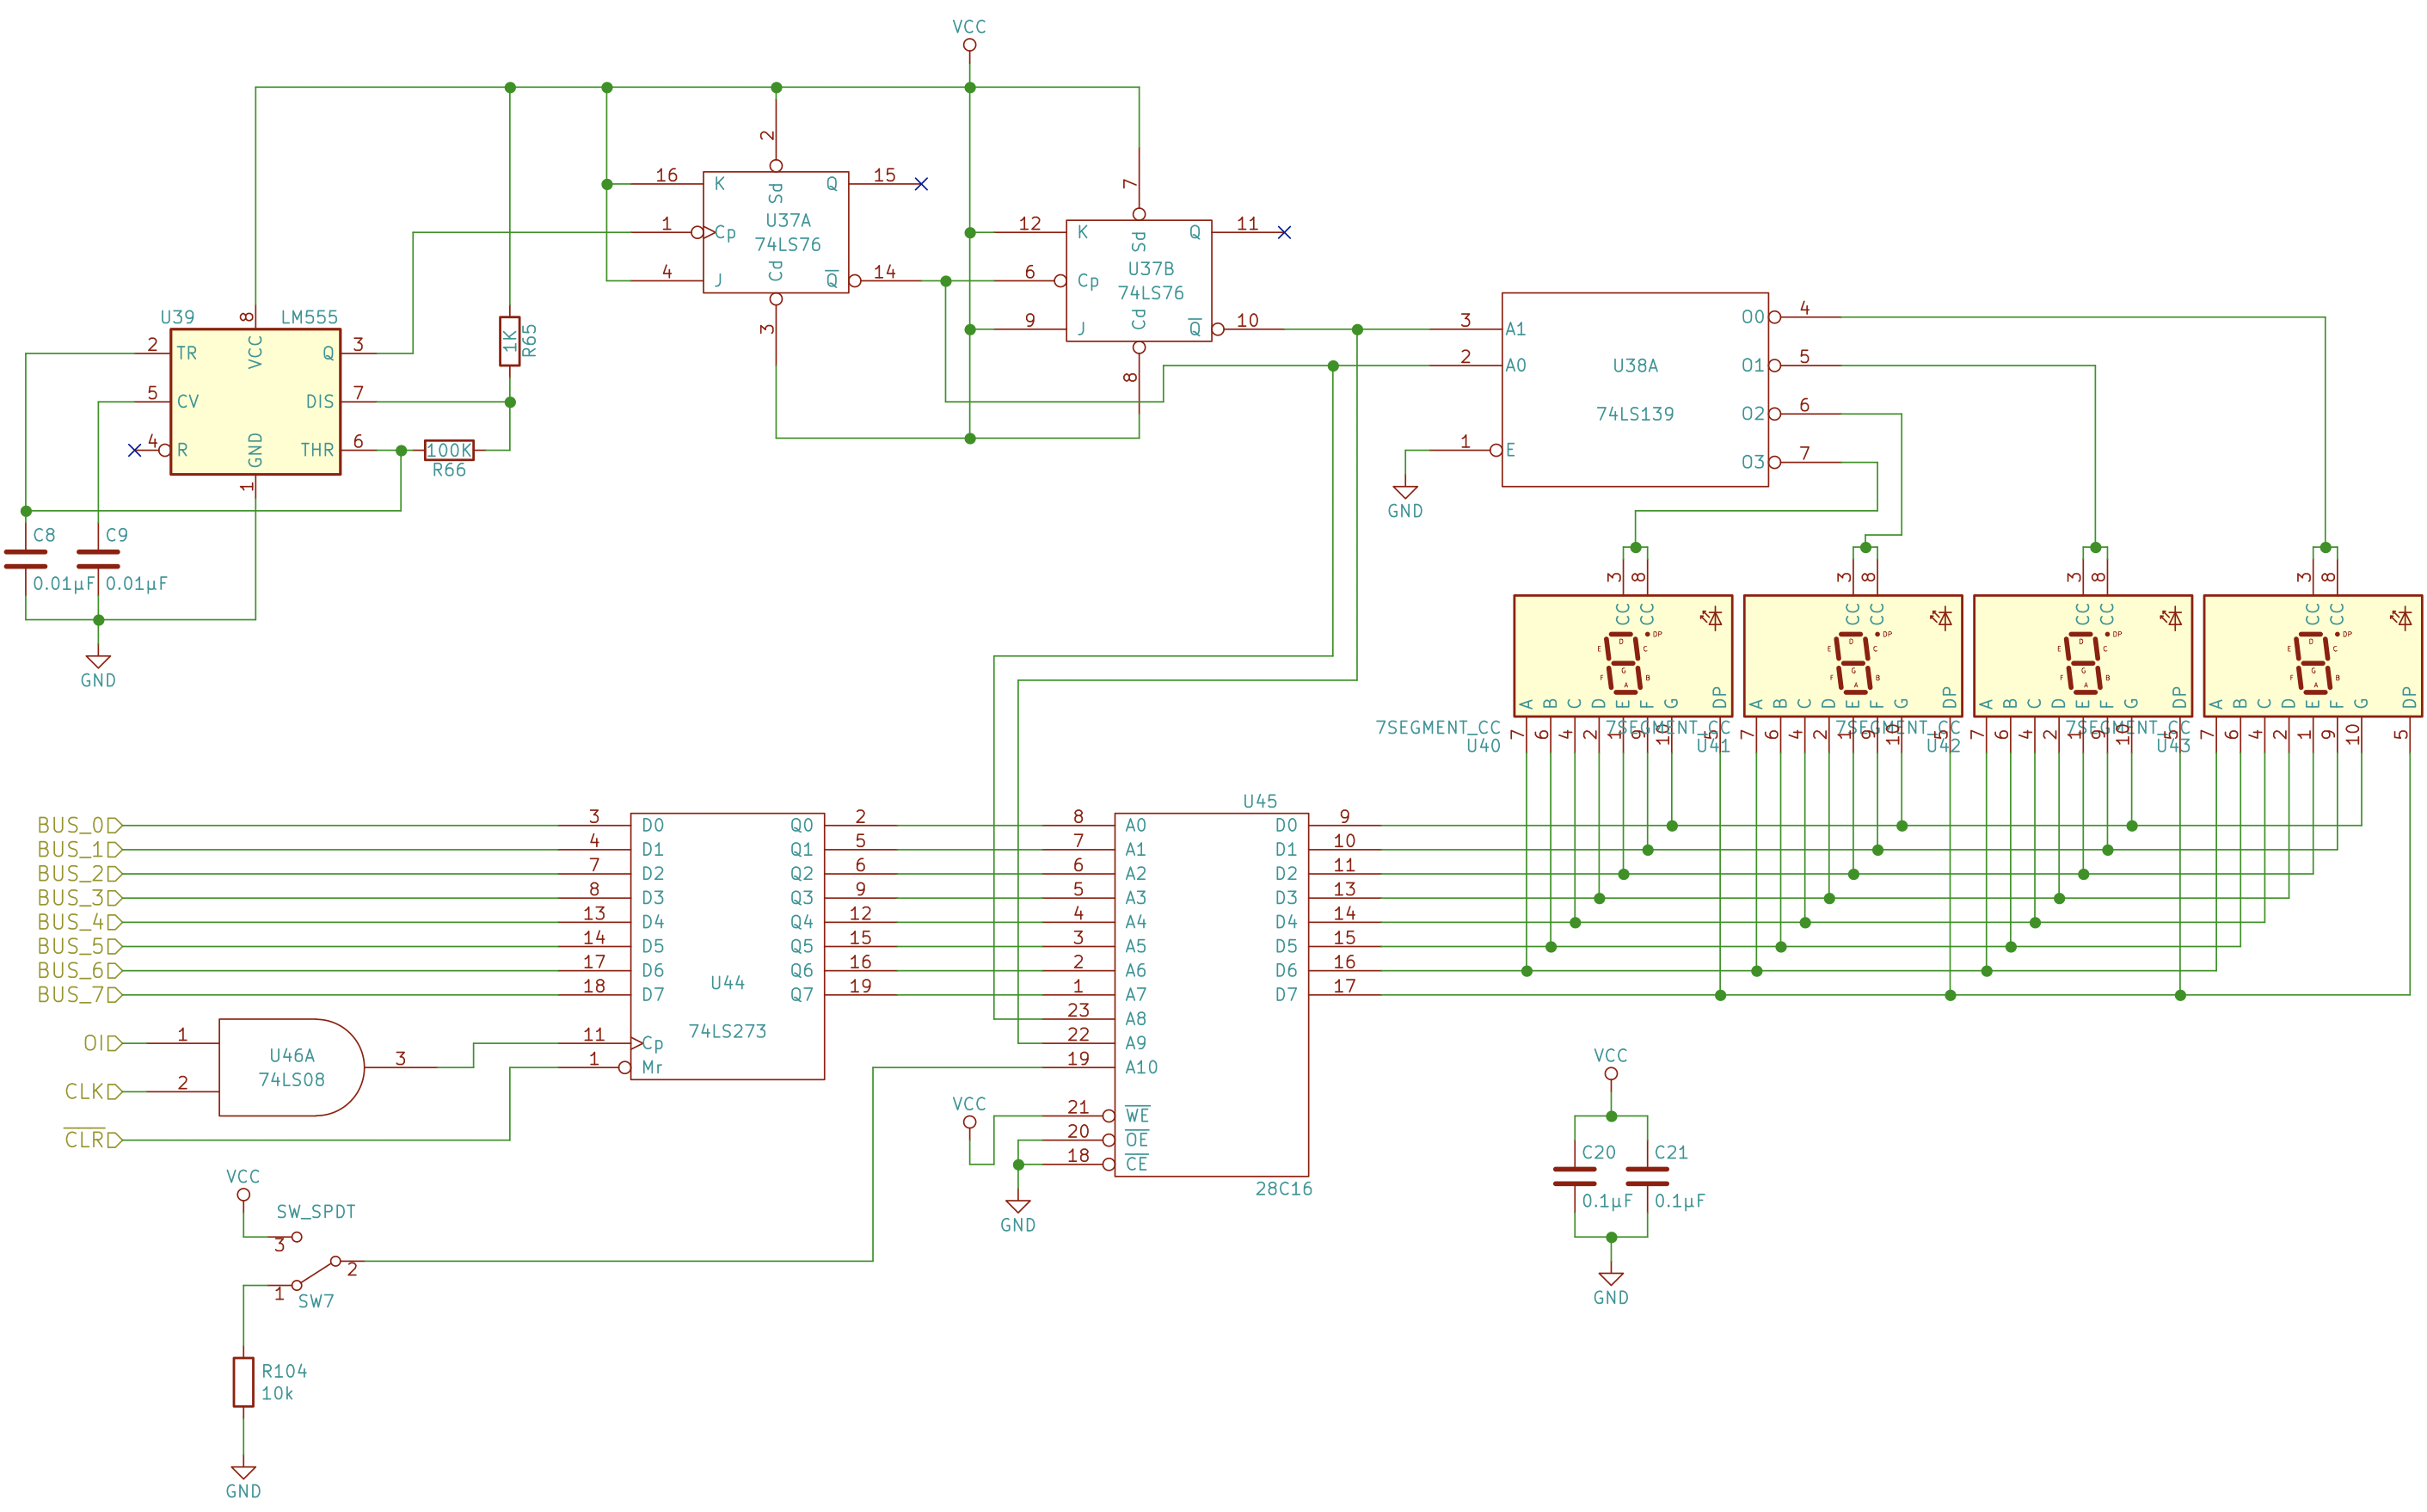
\includegraphics[width=0.7\textwidth]{schematics_output.png}}
  \caption{\label{schematics_output} Esquema do Registrador Output} 
\end{figure}

% \subsubsection{Unidade Central de Processamento (CPU)}
% A lógica de controle é o coração da CPU, é o que define os códigos de operação (opcode) que o processador reconhece e o que acontece quando ele executa cada instrução.

\subsection{Considerações Finais}

Como poder ser observado ao longo do capítulo a implementação do computador é um ponto forte a respeito da compreensão do funcionamento do computador clássico. As subseções apresentadas dão conta do panorama da complexidade, porém, explicam bem o funcionamento de cada módulo, assim bem como a fase de execução de tais.

Apesar do grande avanço na implementação deste computador, muitas partes ainda estão pendentes, conforme já citado no início do capítulo. Todo o esforço empregado até aqui poderá ser utilizado numa possível extensão, caso o tempo de projeto não seja o suficiente. É ressaltado a importância prática de fazer um projeto como esse.


\newpage


